% Seção 7: Circuito de acionamento do aquecedor

\section{Circuito de acionamento do aquecedor}
\label{sec:acionamento}

O circuito de acionamento é mostrado na Figura~\ref{fig:esq_acion}.

\begin{figure}[H]
  \centering
  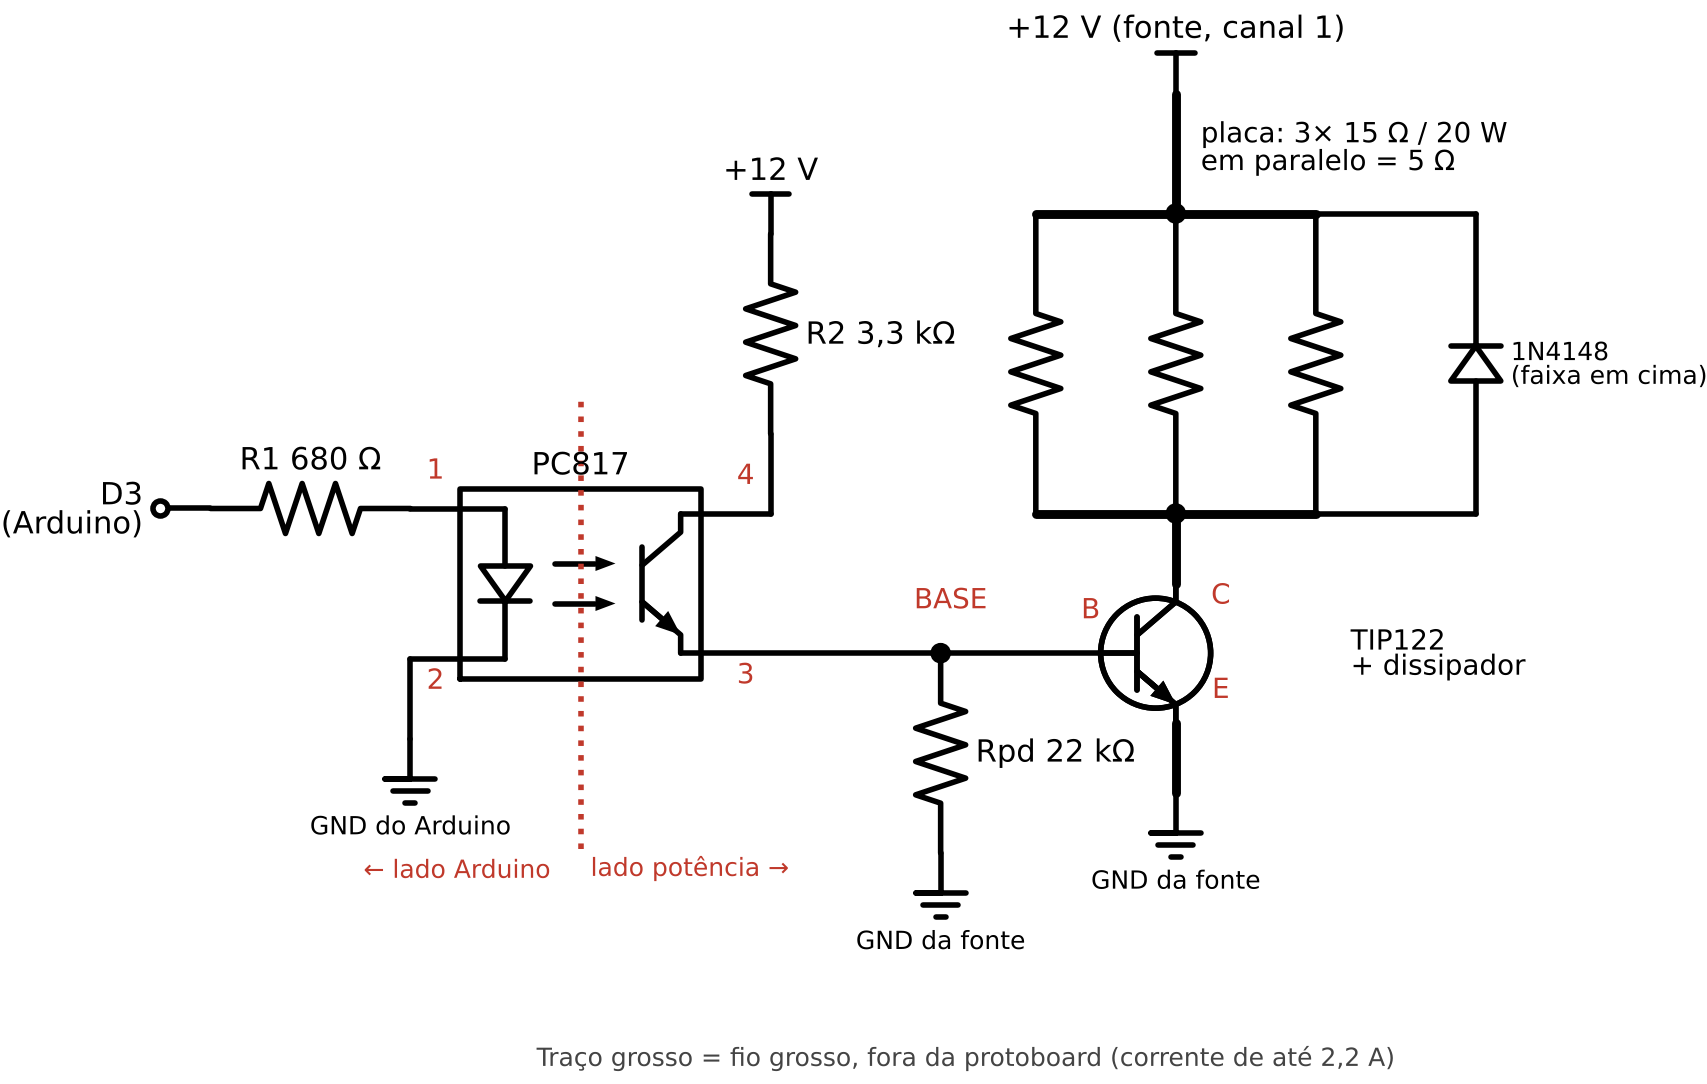
\includegraphics[width=0.9\textwidth]{esq_acionamento.png}
  \caption{Acionamento do aquecedor: optoacoplador PC817, transistor Darlington TIP122 e placa com três resistores de 15\,$\Omega$ em paralelo, alimentada em 12\,V. A linha pontilhada separa os dois lados isolados.}
  \label{fig:esq_acion}
\end{figure}

\paragraph{Optoacoplador.} O pino D3 do Arduino aciona o LED do PC817 por meio de $R_1$ = 680\,$\Omega$:
\begin{equation}
  I_F = \frac{5 - 1{,}2}{680} \approx 5{,}6\ \text{mA}.
\end{equation}
Considerando a razão de transferência de corrente (CTR) mínima de 50\,\%, o fototransistor conduz pelo menos 2,8\,mA. O resistor $R_2$ = 3,3\,k$\Omega$ ligado a 12\,V limita essa corrente a no máximo cerca de 3,1\,mA. O optoacoplador isola eletricamente o Arduino do circuito de potência, e cada lado tem a sua própria referência de terra.

\paragraph{TIP122.} Para a corrente de coletor de 2,2\,A e ganho mínimo $h_{FE} = 1000$, a corrente de base necessária é de
\begin{equation}
  I_B \geq \frac{2{,}2}{1000} \approx 2{,}2\ \text{mA},
\end{equation}
inferior aos cerca de 2,7\,mA fornecidos pelo optoacoplador no caso mais desfavorável, já descontada a corrente desviada pelo \textit{pull-down}. Como a folga é pequena, a saturação será verificada na montagem medindo $V_{CE}$; se passar de cerca de 2\,V, $R_1$ será reduzido para 330\,$\Omega$. O resistor de \textit{pull-down} de 22\,k$\Omega$ mantém o transistor em corte quando o optoacoplador está desligado, inclusive durante a inicialização do Arduino.

\paragraph{Dissipação.} Por ser um Darlington, o TIP122 saturado apresenta queda de tensão de aproximadamente 1,1\,V. A potência dissipada com PWM em 100\,\% é de cerca de $1{,}1 \times 2{,}2 \approx 2{,}5$\,W. Sem dissipador (resistência térmica junção-ambiente de 62,5\,\ensuremath{^\circ}C/W), a elevação de temperatura passaria de 150\,\ensuremath{^\circ}C. Por isso, o TIP122 é montado em um dissipador TO-220 com pasta térmica, que é obrigatório nesta aplicação. Como a aba do TIP122 é ligada ao coletor, o dissipador não pode encostar em outras partes metálicas.

\paragraph{Montagem do circuito de potência.} O caminho da corrente do aquecedor (fonte, placa, TIP122 e retorno) não passa pela protoboard, cujos contatos não suportam 2,2\,A com segurança. Ele é montado com fio de pelo menos 0,5\,mm$^2$ em uma barra de terminais, onde também é fixado o TIP122. Apenas a ligação da base vem da protoboard.

\paragraph{Proteções e PWM.} O diodo 1N4148 em antiparalelo com o aquecedor limita a sobretensão causada pela indutância parasita dos resistores no desligamento; a energia envolvida ($\tfrac{1}{2} L I^2 \approx 5\,\mu$J para $L \approx 2\,\mu$H) é pequena para o diodo. O protetor térmico KSD301, se disponível, fica em série com o aquecedor e interrompe a alimentação acima de 70\,\ensuremath{^\circ}C. O PWM padrão do pino D3 (490\,Hz) é adequado, pois a dinâmica térmica é muito mais lenta que o período de chaveamento. A ventoinha é alimentada diretamente pelo canal 2 da fonte, em 12\,V, e opera com rotação constante.

{\color{red}\noindent\textbf{[A FAZER: refazer as simulações no LTspice com os componentes finais (arquivos em \texttt{simulacoes\_ltspice\_final.zip}): novo print do esquemático do circuito 1 e novos prints do esquemático e das formas de onda do circuito 2. Os números do texto já correspondem aos componentes finais.]}}
